\chapter{Title of first chapter}
\label{chap:Title of first chapter}

Brief summary of this chapter here.

%%%%%%%%%%%%%%%%%%%%%%%%%%%%%%%%%%%%%%%%%%%%%%%%%%%%%%%%%%%%%%%%%%%%%%%%%%%%%%%%
\section{Introduction}
%%%%%%%%%%%%%%%%%%%%%%%%%%%%%%%%%%%%%%%%%%%%%%%%%%%%%%%%%%%%%%%%%%%%%%%%%%%%%%%%

Text here.

\begin{figure}[h]
    \centering
    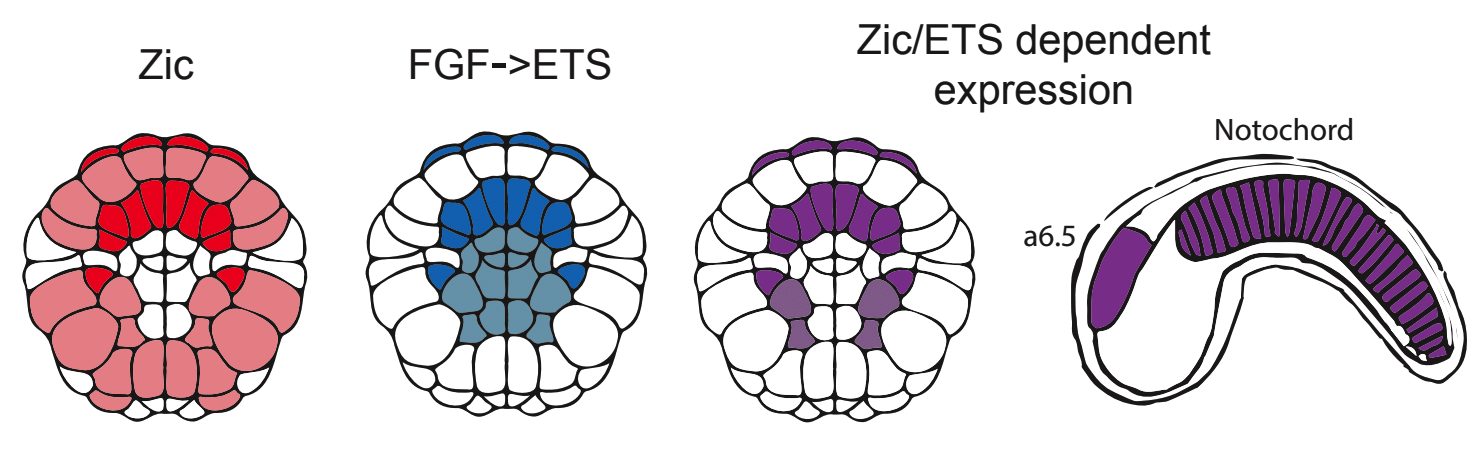
\includegraphics[scale=0.25]{1_figures-and-files/Fig1_ZicEts-Expression.png}
    \caption[Figure caption title.]{\textbf{Figure caption detailing subpanels as necessary.}}
    \label{fig:1 figure title for table of contents}
\end{figure}

%%%%%%%%%%%%%%%%%%%%%%%%%%%%%%%%%%%%%%%%%%%%%%%%%%%%%%%%%%%%%%%%%%%%%%%%%%%%%%%%
\section{Results}
%%%%%%%%%%%%%%%%%%%%%%%%%%%%%%%%%%%%%%%%%%%%%%%%%%%%%%%%%%%%%%%%%%%%%%%%%%%%%%%%

\subsection{Subsection title}

Text here.

%%%%%%%%%%%%%%%%%%%%%%%%%%%%%%%%%%%%%%%%%%%%%%%%%%%%%%%%%%%%%%%%%%%%%%%%%%%%%%%%
\section{Discussion}
%%%%%%%%%%%%%%%%%%%%%%%%%%%%%%%%%%%%%%%%%%%%%%%%%%%%%%%%%%%%%%%%%%%%%%%%%%%%%%%%

In this study \ldots

\subsection{Subsection title}

%%%%%%%%%%%%%%%%%%%%%%%%%%%%%%%%%%%%%%%%%%%%%%%%%%%%%%%%%%%%%%%%%%%%%%%%%%%%%%%%
\section{STAR*Methods}
%%%%%%%%%%%%%%%%%%%%%%%%%%%%%%%%%%%%%%%%%%%%%%%%%%%%%%%%%%%%%%%%%%%%%%%%%%%%%%%%

%%% %%% %%% %%% %%% %%% %%% %%% %%% %%% %%% %%% %%% %%% %%% %%% %%% %%% %%% %%%
\subsection{Key resources table}

\begin{landscape} % this table is long, so it'll be multi-page landscape
    \begin{longtable}{p{.49\textwidth} p{.35\textwidth} p{.5\textwidth}}
        % Define the table title in the table of contents
        \caption{Key resources table} \\ \hline 

        % Define the table columns for the first and all subsequent pages
        \multicolumn{1}{l}{\textbf{REAGENT or RESOURCE}} & \multicolumn{1}{l}{\textbf{SOURCE}} & \multicolumn{1}{l}{\textbf{IDENTIFIER}} \\ \hline \endfirsthead

        \multicolumn{3}{l}%
        {{\textbf{\tablename\ \thetable{}.} Key resources table, \textit{continued from previous page}}} \\
        \hline 
        \multicolumn{1}{l}{\textbf{REAGENT or RESOURCE}} & \multicolumn{1}{l}{\textbf{SOURCE}} & \multicolumn{1}{l}{\textbf{IDENTIFIER}} \\ \hline\hline \endhead

        % Define the table footer for the first and all subsequent pages
        \hline \multicolumn{3}{r}{\textit{Continued on next page}} \\ \hline \endfoot
        \hline \endlastfoot
        
        % Start table content

        %%%%% %%%%% %%%%% %%%%% %%%%% %%%%% %%%%% %%%%% %%%%% %%%%% %%%%% %%%%%
        \textit{Deposited Data} \\ \hline
        Data Info \\ 
        Data Info \\
        Data Info \\
        Data Info \\
        Data Info \\
        Data Info \\
        Data Info \\
        
        %%%%% %%%%% %%%%% %%%%% %%%%% %%%%% %%%%% %%%%% %%%%% %%%%% %%%%% %%%%%
        \hline \textit{Experimental Models: Organisms/Strains} \\ \hline
        \textit{Ciona} intestinalis type A (\textit{Ciona} robusta) & M-Rep & N/A \\

        %%%%% %%%%% %%%%% %%%%% %%%%% %%%%% %%%%% %%%%% %%%%% %%%%% %%%%% %%%%%
        \hline \textit{Oligonucleotides} \\ \hline
        Oligonucleotides for library screen, see Table S1 & This paper & N/A \\
        Oligonucleotides for mutagenesis, see Table S4 & This paper & N/A \\

        %%%%% %%%%% %%%%% %%%%% %%%%% %%%%% %%%%% %%%%% %%%%% %%%%% %%%%% %%%%%
        \hline \textit{Recombinant DNA} \\ \hline
        Plasmid: BraS bpFog$>$GFP & Farley Lab & N/A \\ 
        Plasmid: BraS -ZEE bpFog$>$GFP & This paper & N/A \\
        Plasmid: BraS rZE bpFog$>$GFP & This paper & N/A \\
        Plasmid: BraS -FoxA bpFog$>$GFP & This paper & N/A \\
        Plasmid: BraS -Bra bpFog$>$GFP & This paper & N/A \\ 
        Plasmid: BraS rZEFB bpFog$>$GFP & This paper & N/A \\
        Plasmid: Lama1 bpFog$>$GFP & This paper & N/A \\
        Plasmid: Lama1 bpFog$>$GFP & This paper & N/A \\
        Plasmid: Lama1 -E3 bpFog$>$GFP & This paper & N/A \\
        Plasmid: Lama1 -Z bpFog$>$GFP & This paper & N/A \\
        Plasmid: Lama1 RE3 bpFog$>$GFP & This paper & N/A \\

        %%%%% %%%%% %%%%% %%%%% %%%%% %%%%% %%%%% %%%%% %%%%% %%%%% %%%%% %%%%%
        \hline \textit{Software and Algorithms} \\ \hline
        Python (version 3.8.6)  & Python Software Foundation & \href{https://www.python.org}{https://www.python.org} \\
        Conda (version 4.9.2) & Anaconda, Inc. & \href{https://docs.conda.io/}{https://docs.conda.io} \\
        Bioconda  & Grüning et al., 2018 & \href{https://bioconda.github.io}{https://bioconda.github.io} \\
        Biopython (version 1.78) & Cock et al., 2009 & \href{https://biopython.org}{https://biopython.org} \\
        FastQC (version 0.11.9)	& Babraham Institute & \href{https://www.bioinformatics.babraham.ac.uk/}{https://www.bioinformatics.babraham.ac.uk} \\
        MultiQC (version 1.8) & Ewels et al., 2016 & \href{https://multiqc.info}{https://multiqc.info} \\
        FLASH (version 1.2.11) & Magoč et al., 2011 & \href{http://www.cbcb.umd.edu/software/flash}{http://www.cbcb.umd.edu/software/flash} \\
        \verb|pandas| (version 1.2.1) & NumFOCUS & \href{https://pandas.pydata.org}{https://pandas.pydata.org} \\
        \verb|numpy| (version 1.20.3) & Harris et al., 2020 & \href{https://numpy.org}{https://numpy.org} \\
        \verb|matplotlib| (version 3.2.2) & Hunter, 2007 & \href{https://matplotlib.org/}{https://matplotlib.org} \\
        \verb|scikit-learn| (version 0.24.1) & Pedregosa et al., 2011 & \href{https://scikit-learn.org/}{https://scikit-learn.org} \\
        \verb|seaborn| (version 0.11.1) & Waskom et al., 2021 & \href{https://seaborn.pydata.org/}{https://seaborn.pydata.org} \\
        \verb|Diverse-Logics-Notochord-Study| & Code used in this paper & \href{https://github.com/Github/RepoName}{RepoName Github} \\
    \end{longtable}
\end{landscape}

%%% %%% %%% %%% %%% %%% %%% %%% %%% %%% %%% %%% %%% %%% %%% %%% %%% %%% %%% %%%
\subsection{Resource availability}

%%% %%% %%% %%% %%% %%% %%% %%% %%% %%% %%% %%% %%% %%% %%% %%% %%% %%% %%% %%%
\subsubsection{Lead contact} 
Further information and requests for resources and reagents should be directed to and will be fulfilled by the lead contact, Professor One (\href{mailto:email@gmail.com}{email@gmail.com}). 

%%% %%% %%% %%% %%% %%% %%% %%% %%% %%% %%% %%% %%% %%% %%% %%% %%% %%% %%% %%%
\subsubsection{Materials availability} 
Plasmids generated in this study are available upon request. 

%%% %%% %%% %%% %%% %%% %%% %%% %%% %%% %%% %%% %%% %%% %%% %%% %%% %%% %%% %%%
\subsection{Experimental model and subject details}
\subsubsection{Tunicates}
Adult \textit{\textit{Ciona} intestinalis type A}, also known as \textit{\textit{Ciona} robusta}, were obtained from M-Rep and were maintained under constant illumination in seawater (obtained from Reliant Aquariums) at $18^\circ$C. \textit{Ciona} are hermaphroditic, therefore there is only one possible sex for individuals. Age or developmental stage of the embryos studied are indicated in the main text. 

%%% %%% %%% %%% %%% %%% %%% %%% %%% %%% %%% %%% %%% %%% %%% %%% %%% %%% %%% %%%
\subsection{Method details}
\subsubsection{Library Construction}
Details here.

\subsubsection{GFP reporter assays}
Details here.


%%%%%%%%%%%%%%%%%%%%%%%%%%%%%%%%%%%%%%%%%%%%%%%%%%%%%%%%%%%%%%%%%%%%%%%%%%%%%%%%
\section{Data and code availability}
%%%%%%%%%%%%%%%%%%%%%%%%%%%%%%%%%%%%%%%%%%%%%%%%%%%%%%%%%%%%%%%%%%%%%%%%%%%%%%%%

Any additional information required to reanalyze the data reported in this paper is available from the lead contact upon request. 

%%%%%%%%%%%%%%%%%%%%%%%%%%%%%%%%%%%%%%%%%%%%%%%%%%%%%%%%%%%%%%%%%%%%%%%%%%%%%%%%
\section{Acknowledgments}
%%%%%%%%%%%%%%%%%%%%%%%%%%%%%%%%%%%%%%%%%%%%%%%%%%%%%%%%%%%%%%%%%%%%%%%%%%%%%%%%

We thank \dots for helpful discussions and comments on the manuscript. This work was supported by \dots.

% Include the acknowledgement that this is a reformatted reprint
Chapter 1,  in full,  is  a  reformatted  reprint  of  the  material as it appears in “Paper title”  Author A. One, Author B. Two. \textit{Science}, 2023.  The dissertation author was the primary investigator and co-first author of this paper.

%%% %%% %%% %%% %%% %%% %%% %%% %%% %%% %%% %%% %%% %%% %%% %%% %%% %%% %%% %%%
\subsection{Author contributions}
A.A.O. designed experiments. A.A.O. and A.B.T. conducted experiments. A.A.O. analyzed data. A.A.O. and A.B.T. wrote the manuscript.

%%% %%% %%% %%% %%% %%% %%% %%% %%% %%% %%% %%% %%% %%% %%% %%% %%% %%% %%% %%%
\subsection{Declaration of interests}
The authors declare no competing interests.
